\section{Evaluation}
\label{sec:Evaluation}

\textbf{General procedure:}We used Alam et al.'s approach to instrument a PivotPaths visualization ~\cite{dork2012pivotpaths} of movie data extracted from the Internet Movie DataBase (IMDB). We used this instrumented system to collect DOI data from 9 subjects, solving a range of tasks such as identifying similarities between two movies, using three movie titles to recommend a fourth, and ranking the degree to which directors collaborated with certain actors. We then created a visualization that could show DOI data coming from multiple users concurrently in real-time. We invited eleven subjects to analyse the collected DOI data. Five of these subjects analyzed the data in a simulated real-time scenario: we streamed the previously collected DOI through our visualization little by little, as if it was captured concurrently from multiple users right then. The other six subjects analyzed the same DOI data but in an offline-scenario, meaning that subjects were shown all data from the beginning rather through streaming. We asked all our eleven subjects to indentify what tasks their monitored users were doing, and compared their answers to the real task descriptions.

\textbf{PivotPaths visualization:}Our instrumented visualization system allowed its users to search for movies, actors, or directors, and created diagrams which displayed movies, actors, directors, and genres most closely related to the searched items, and connections between them, using a layout exemplified in Figure~\ref{fig:pivotpaths}. The system's rendering code was instrumented using Alam et al.'s approach such as to capture what movies, actors, directors, or genres users viewed at each moment in time. The temporal resolution was determined by the eye-tracker's sampling frequency.

\textbf{Collecting DOI data:} We collected DOI data from 9 graduate and undergraduate students solving movie related task using the system described above. We used a light weight 60Hz EyeX Tobii eye-tracker. Users were payed \$10 for their effort. After introductory and training sessions in which we taught users how to interpret and interact with the PivotPaths visualization, we asked users to complete the tasks listed below. We will name and number these tasks as ``data collection tasks'' (DC tasks).
\begin{itemize}
	\item DC\_Task1: Given two movie titles, ``Raiders of the lost ark'' and ``Indiana Jones and the last Crusade'', find two actors, two genres, and one director they have in common. 
	\item DC\_Task2: Given a director name, James Cameron, and a list of three actors, ``Arnold Schwarzenegger'', ``Linda Hamilton'', and ``Sigourney Weaver'', rank the actors in terms of their collaboration with the director. 
	\item DC\_Task3: Given three movie titles, ``Catch me if you can'', ``E.T.: The extra-terrestrial'', and ``Captain Phillips'', recommend a fourth movie. 
\end{itemize}

 
\textbf{Visualizing DOI data:}  Our visualization of streaming eye-tracking data combined elements of heatmap and time-line representations Figure~\ref{fig:heatmap}. Given the current time $t$ in a user's DOI stream, we identified the ten data objects that user viewed most in the recent $t-90$second time span. We created heatmap representations which list those ten objects vertically, show time horizontally in $1$ second increments, and color cells based on the amount of interest shown for a particular object at a particular time. The data objects featured in the heatmap were ordered vertically and scaled based on the amount of interest the user expressed in them in the considered $t-90$second time span. We stacked such matrices on top of each other, one for each individual user.

\textbf{Interpreting DOI data in real-time, a user study:} We invited 10 subjects, two males and eight females, to participate in a data analysis (DA) user study in which we assessed their ability to intepret the collected DOI data. We gave our DA subjects an incomplete definition of the tasks that the DC users had to do, used the visualization in Figure~\ref{fig:heatmap} to show them data from five users (we used the remaining four data sets for training), and asked them to use this data to fill in the missing details in the incomplete task descriptions. Moreover, we randomized the order in which each of our DC users completed their three tasks, and asked our data analysts to poinpoint the time when each of their monitored users started a new task. Specifically, we gave analysts the following four tasks:  
\begin{itemize}
	\item DA\_Task1: For each featured user, indicate when they are starting a new task and what that task is.
	\item DA\_Task2: Knowing the movie title of DC\_Task 1, identify the common elements that DC users would have found (two actors, two genres, one director).
	\item DA\_Task3: Knowing the director name in DC\_Task2, identify the the three actors named in the task.
	\item DA\_Task4: Knowing the three movies involved in DC\_Task3, identify the movie that users would have found. 

\end{itemize}

As described previously, five of our analysts saw all their users data at once, replicating an offline analysis, while for the remaining five we simulated an online scenario  by streaming our collected data gradually. We hypothesized that our offline analysts will provide more accurate results because of their ability to analyze the entire data at once at a more leisurely pace. Our design was intended to capture the difference.  

In terms of protocol, each of our subjects was given an introduction to eye-tracking and DOI collection, then was instructed on the procedure used in the DC stage and given their task description (DA tasks). Subjects were then allowed to familiarize themselves with movies involved in their tasks by browsing the IMDB website. This was followed by a training session in which subjects were shown the DOI visualization, and then allowed to view a few minutes worth of data from half of our DC users. Finally, we conducted the actual study using the remaining data collected from our DC users.   The offline session lasted for about one hour while the real-time session for about fifty minutes. All subjects were awarded \$10 for their time.



\begin{figure}[htb]
  \centering
  \includegraphics[width=\linewidth]{images/pivotpaths.eps}
  \caption{PivotPaths visualization of IMDB data. Movies are displayed in the center of the screen, actors at the top, and directors and genres share the bottom space. Actors, directors, and genres associated to movies are connected through curves. Users can highlight objects and their connected neighbors by hovering over them.}
	\label{fig:pivotpaths}
\end{figure}

\begin{figure}[htb]
  \centering
  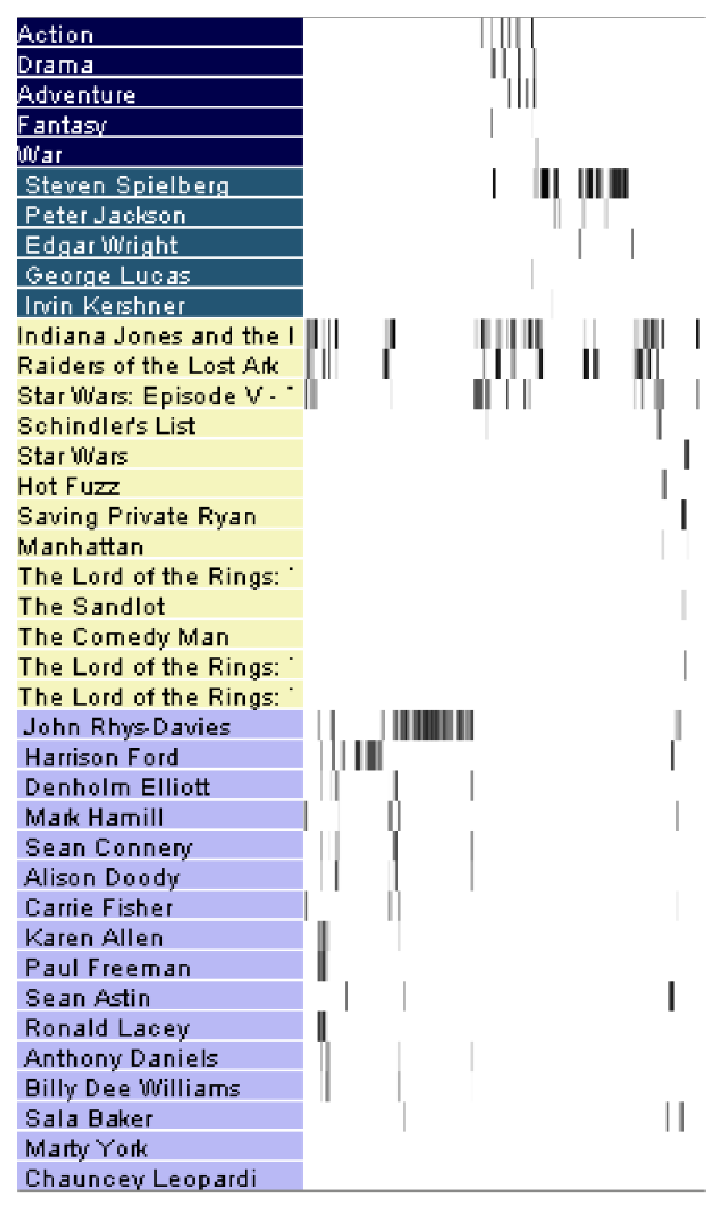
\includegraphics[width=\linewidth]{images/heatmap.eps }
  \caption{A time-line visualization of DOI data streaming from multiple users concurrently. For each user, the ten most viewed objects in the last $90$ seconds are listed vertically, ordered and scaled by the amount of interest the user showed in them. Time advances horizontally (most recent moment on the right), and the degree to which each object was viewed in each $1$ second time step is captured by color.}
	\label{fig:heatmap}
\end{figure}


